%%%%%%%%%%%%%%%%%%%%%%%%%%%%%%%%%%%%%%%%%
% Journal Article
% LaTeX Template
% Version 1.4 (15/5/16)
%
% This template has been downloaded from:
% http://www.LaTeXTemplates.com
%
% Original author:
% Frits Wenneker (http://www.howtotex.com) with extensive modifications by
% Vel (vel@LaTeXTemplates.com)
%
% License:
% CC BY-NC-SA 3.0 (http://creativecommons.org/licenses/by-nc-sa/3.0/)
%
%%%%%%%%%%%%%%%%%%%%%%%%%%%%%%%%%%%%%%%%%

%----------------------------------------------------------------------------------------
%	PACKAGES AND OTHER DOCUMENT CONFIGURATIONS
%----------------------------------------------------------------------------------------

\documentclass[twoside,twocolumn]{article}

\usepackage{blindtext} % Package to generate dummy text throughout this template 

\usepackage[sc]{mathpazo} % Use the Palatino font
\usepackage[T1]{fontenc} % Use 8-bit encoding that has 256 glyphs
\linespread{1.05} % Line spacing - Palatino needs more space between lines
\usepackage{microtype} % Slightly tweak font spacing for aesthetics

\usepackage[english]{babel} % Language hyphenation and typographical rules

\usepackage[hmarginratio=1:1,top=32mm,columnsep=20pt]{geometry} % Document margins
\usepackage[hang, small,labelfont=bf,up,textfont=it,up]{caption} % Custom captions under/above floats in tables or figures
\usepackage{booktabs} % Horizontal rules in tables

\usepackage{lettrine} % The lettrine is the first enlarged letter at the beginning of the text

\usepackage{enumitem} % Customized lists
\setlist[itemize]{noitemsep} % Make itemize lists more compact

\usepackage{abstract} % Allows abstract customization
\renewcommand{\abstractnamefont}{\normalfont\bfseries} % Set the "Abstract" text to bold
\renewcommand{\abstracttextfont}{\normalfont\small\itshape} % Set the abstract itself to small italic text

\usepackage{titlesec} % Allows customization of titles
\renewcommand\thesection{\Roman{section}} % Roman numerals for the sections
\renewcommand\thesubsection{\roman{subsection}} % roman numerals for subsections
\titleformat{\section}[block]{\large\scshape\centering}{\thesection.}{1em}{} % Change the look of the section titles
\titleformat{\subsection}[block]{\large}{\thesubsection.}{1em}{} % Change the look of the section titles

\usepackage{fancyhdr} % Headers and footers
\pagestyle{fancy} % All pages have headers and footers
\fancyhead{} % Blank out the default header
\fancyfoot{} % Blank out the default footer
\fancyhead[C]{Running title $\bullet$ May 2016 $\bullet$ Vol. XXI, No. 1} % Custom header text
\fancyfoot[RO,LE]{\thepage} % Custom footer text

\usepackage{titling} % Customizing the title section

\usepackage{hyperref} % For hyperlinks in the PDF

\usepackage{graphicx}

%----------------------------------------------------------------------------------------
%	TITLE SECTION
%----------------------------------------------------------------------------------------

\setlength{\droptitle}{-4\baselineskip} % Move the title up

\pretitle{\begin{center}\Huge\bfseries} % Article title formatting
\posttitle{\end{center}} % Article title closing formatting
\title{Article Title} % Article title
\author{%
\textsc{Frederik Vincent Primdahl} \textsc{Mikael Steenberg Pasovski} \and \textsc{Andreas Peter Brodersen} \textsc{Andreas Wede Gustavsen} \\[1ex] % Your name
\normalsize Copenhagen School of Design and Technology \\ % Your institution
%\and % Uncomment if 2 authors are required, duplicate these 4 lines if more
%\textsc{Jane Smith}\thanks{Corresponding author} \\[1ex] % Second author's name
%\normalsize University of Utah \\ % Second author's institution
%\normalsize \href{mailto:jane@smith.com}{jane@smith.com} % Second author's email address
}
\date{\today} % Leave empty to omit a date
\renewcommand{\maketitlehookd}{%
\begin{abstract}
In this paper data gathered from product reviews on the e-commerce site Amazon.com is assessed to discover if the helpfulness of a review can be determined from the frequency of words used. Using the amount of votes a review has received as an indicator of helpfulness, text classification is done to group a review into one of two classes – helpful or unhelpful. We argue that parameterizing text data by term-frequency vastly improves predictions compared to an inverse term-frequency statistic, and that some classifiers perform better when only a few features are used, but that involving more features would likely improve performance overall. Finally, we find that predicting the helpfulness of a review based on votes is difficult, as the dataset provided is biased in the favor of unhelpful reviews, making the likelihood of helpful terms appearing in reviews with no votes very high.
\end{abstract}
}

%----------------------------------------------------------------------------------------

\begin{document}

% Print the title
\maketitle

%----------------------------------------------------------------------------------------
%	ARTICLE CONTENTS
%----------------------------------------------------------------------------------------

\section{Introduction}
In the globalized economy of today, consumers are presented with a range of products to choose from when shopping. This can present some difficulty, as quality of the product is not always clear from its presentation. The customer review seeks to solve this by providing feedback on the purchase. Still, determining the value of a review can be difficult, as reviews can be misleading or provide little information.

Voting systems are often set in place to identify helpful reviews, and help consumers circumvent this issue, yet these reviews still get lost in the sheer number of unlabeled reviews. Our machine learning model aims to further filter reviews mainly by analyzing use of words, verbosity, among other aspects, to discover what makes a review helpful.

%------------------------------------------------
\section{Problem Formulation}

The main focus of this paper is to analyze Amazon review data across different categories and answer the question: “To what extent can the helpfulness of an Amazon review be predicted?” through the use of classification models.

%------------------------------------------------
\section{Methods}
Our research aims at creating a predictive model for identifying helpful Amazon reviews. Therefore, the data used in this study is a subset of Amazon product reviews divided into categories, with each product and reviewer having at least 5 reviews.

As our model is primarily trained on text data, common Natural Language Processing techniques have been used in the preprocessing of data and the subsequent structuring of this data into input data.

For converting our text data into parametric data for use in building our model, we have chosen to use document-term matrices through Count Vectorization and TF-IDF Vectorization. By employing two methods of text vectorization, we can more easily determine which term weighing factor improves the most upon the performance metrics of our model.

Since we are dealing with a binary classification problem due to separation of reviews into two groups - helpful and unhelpful - we make use of several different classifiers in training our model. We are labelling each review on its helpfulness feature to make supervised learning through each of these classifiers possible.

For our model evaluation we make use of primarily two statistics. A confusion matrix is used in summarizing the performance of the classifier algorithms used in training our model. As mentioned, we are dealing with a binary classification problem, and as in many problems of this nature, the two groups are not symmetric. Therefore we also apply Youden's Index to make up for our unbalanced dataset, using this statistic as a final measure of our model's predictive power.
\subsection{Data exploration}

With the cleaned up dataset and the research question in mind, columns with relevance are explored. To explore, we plot different columns of interest to identify any patterns in the data in connection to review helpfulness. We plot the distribution between reviews with votes and no votes.
\begin{figure}[h]
	\centering
	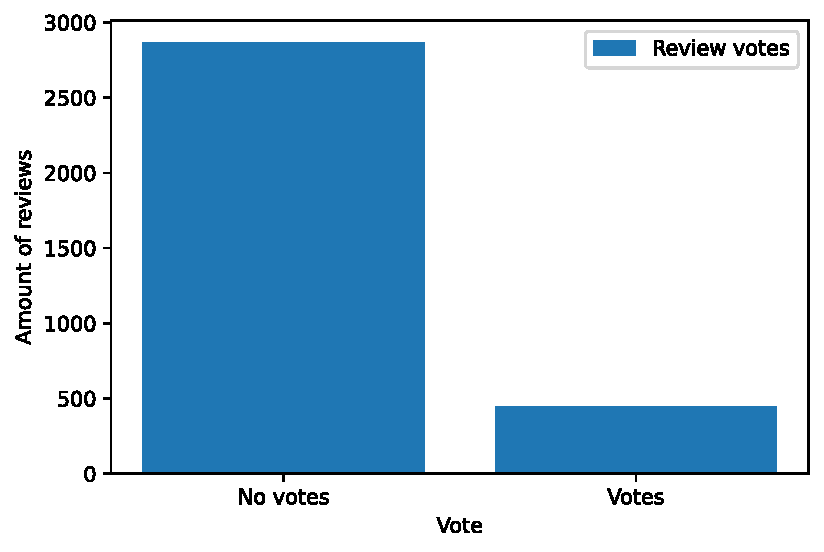
\includegraphics[width=0.5\textwidth]{img/no_votes_vs_votes.pdf}
	\caption{Upvote distribution}
	\label{fig:votes_distribution}
\end{figure}
As seen in \figurename{\ref{fig:votes_distribution}}, the distribution is very uneven in favor of reviews with no votes. This is relevant when evaluating performance metrics of our model, as it indicates that a statistic like Youden's Index might be useful to counteract random guessing. To get another perspective on review votes we plot the data into a heatmap in relation to ratings.
\begin{figure}[h]
	\centering
	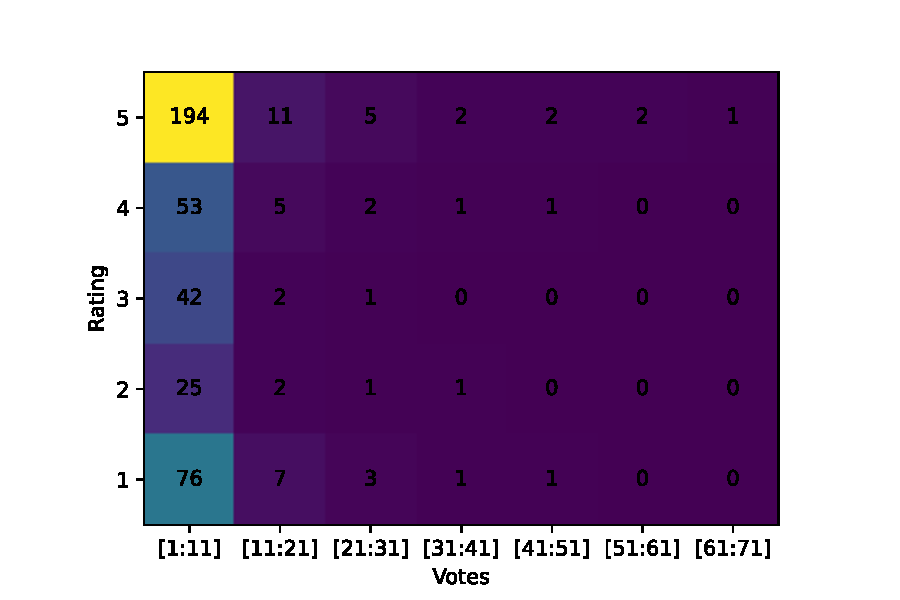
\includegraphics[width=0.5\textwidth]{img/rating_vote_heatmap_excluding_no_votes.pdf}
	\caption{Votes in relation to rating}
	\label{fig:rating_vote_heatmap}
\end{figure}
\figurename{\ref{fig:rating_vote_heatmap}} shows the ratings binned with the amount of votes. This heatmap only shows reviews with votes. The heatmap gives an indication of how votes combined with ratings are distributed in our dataset in a more specific way with the binned votes compared to \figurename{\ref{fig:votes_distribution}}.

%------------------------------------------------

\begin{figure*}[t]
	\centering% Do not use center environment, it adds additional vertical space

	\begin{center}
		\begin{tabular}{||c c c c c c||}
			\hline
			Count/TF-IDF & Classifier  & Train-set size & Parameters     & Time spend            & Youden's Index \\ [0.5ex]

			\hline\hline
			Count        & MLP         & 876.132        & LBFGS, 1x50    & 23min 5sec (i7 8700k) & 0.25646        \\

			\hline
			Count        & MLP         & 241.209        & Adam, 2x100    & 184min 24sec (M1 Air) & 0.23941        \\

			\hline
			Count        & MLP         & 107.302        & LBFGS, 1x100   & 2min 3sec (M1 Air)    & 0.23504        \\

			\hline
			Count        & LogisticReg & 107.302        & max iter=10000 & 17 sec (i7 6700k)     & 0.22513        \\

			\hline
			Count        & MLP         & 107302         & LBFGS, 1x50    & 2min 25sec(M1 Air)    & 0.22214        \\

			\hline
			Count        & SVC         & 107.302        & max iter=5000  & 58sec (M1 Air)        & 0.21384        \\

			\hline
			Count        & MLP         & 107.302        & Adam, 1x100    & 63min 2sec (M1 Air)   & 0.18065        \\

			\hline
			TF-IDF       & LogisticReg & 107.391        & max iter=10000 & 0.3sec (i7 6700k)     & 0.12344        \\

			\hline
			TF-IDF       & SVC         & 107.391        & max iter=5000  & 1.4sec (i7 6700k)     & 0.06107        \\


			\hline
		\end{tabular}
	\end{center}
	\caption{Model test runs}
	\label{model_test_runs}
\end{figure*}

\section{Analysis}

\subsection{Ethics and bias}
As our model seeks to highlight helpful reviews, and distinguish - or filter - these from the unhelpful ones, ethics regarding censorship must be considered. Specific associations with words can often be attributed to bias, making NLP models whose purpose it is to filter undesired text prime censorship tools in the wrong hands\footnote\cite{censorship}. In the context of our model, a very real use-case would be as a tool for preventing unhelpful reviews from being submitted. However, unhelpfulness is subject to opinion, and controversial statements can quickly be tagged as bad and subsequently filtered out.

\subsection{Data Preprocessing}

\begin{figure}[h]
	\centering
	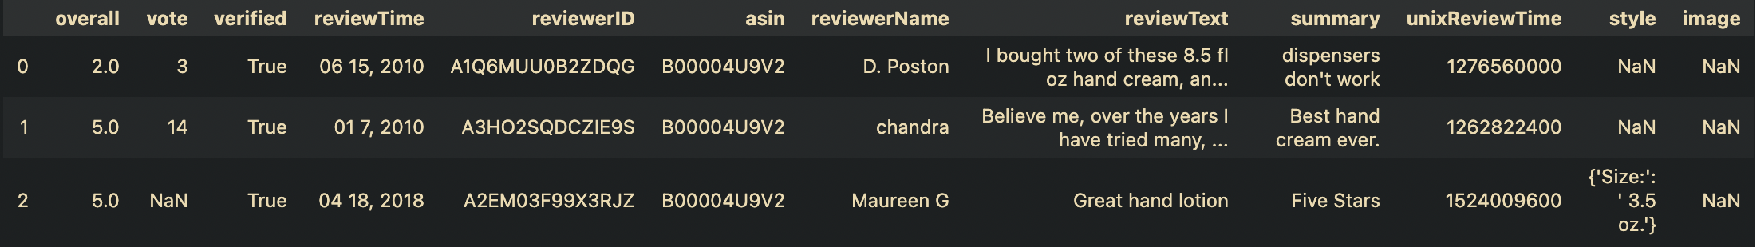
\includegraphics[width=0.5\textwidth]{img/unclean_data.pdf}
	\caption{Unclean data}
	\label{fig:unclean_data}
\end{figure}

Our starting point of data preparation was to understand what an Amazon review consists of. The raw data can be seen in \figurename{\ref{fig:unclean_data}}.

Initial data preparation was carried out on the whole dataset, dropping review time, image, style, ASIN, and reviewer id columns, as these were not needed. Unverified reviews were also filtered out, to avoid reviews from customers who did not purchase the product. Finally, null values were removed from the review text column.

As our input data mainly consists of unstructured text reviews, text normalization\footnote was done on the review text column to reduce randomness and reach a more uniform structure. This was done in accordance with common NLP data cleaning guidelines. Steps in this process involved removing non-word elements from the text – punctuation, symbols -, along with transforming each remaining word into lowercase. Because our model concerns itself with classification rather than sentiment, stop words like “not” did not provide any additional information to our model and were subsequently removed, as with other stop words contained in the NLTK “stopwords” library.

Each review was then tokenized into separate words using whitespace as a delimiter, as part of lemmatization to reduce morphological variation. Shortening some words to their root was thought important to improve model training efficiency. Lemmatization was chosen over stemming, as the accuracy of a lemmatizer in properly shortening words was more important than the speed of a stemmer.

As the next step of our data cleanup a column “voteSuccess” was added to the dataframe, calculating helpfulness of a review by dividing number of votes from the “votes”-column by quarters elapsed since the review was submitted. This was done to create a fairer indicator of helpfulness, since newer reviews would have had less time to accumulate helpfulness-votes and therefore appear less helpful.

For training our model, a numeric representation of our text corpus was needed for providing our models with input data. This was the final part of data preprocessing. Document-term matrices were created from two different vectorizations – Count\footnote and TF-IDF\footnote. Count vectorization parses a text corpus into a matrix based on the frequency of each term occurring in that corpus. This method was therefore the easiest way for us to present our data as something our classifiers could use. To discover if any less informative words not removed as part of our data cleanup were negatively impacting the performance of our model, we also opted for TF-IDF vectorization of our text data. TF-IDF favors unique terms appearing in documents higher, likely leading to a difference in model accuracy and precision metrics, and F1 scores.

\subsection{Model Building}
To begin our model building LinearSVC was chosen as the initial classifier for our dataset. LinearSVC tries to classify our data into two groups, helpful and unhelpful since our problem is of a binary nature, and tries to find the optimal split between these two\cite{sklearn:LinearSVC}. Initially the model did not converge in time. We therefore tried different max iterations to see when the model would converge and avoid overfitting and find the best fit for classifying a review as helpful/unhelpful. Performance does take a hit as the data size increases, see \figurename{\ref{model_test_runs}}.

After trying SVM as our first classifier, we wanted to try a neural network on the dataset. Both SVM and neural network seemed like a great place to start, since they can be used in most machine learning tasks and yield decent results.

We've used the Multi-layer Perceptron classifier with different amounts of hidden layers, nodes and solvers.

During our testing the performance scaled positively as the size of the dataset increased. The cost of using the Adam solver over the LBFGS is higher, increasing the fitting dramatically as the training set grows, which matches scikit-learn's documentation\cite{sklearn:MLPClassifier}.

Playing around with the nodes and layers got us to the ideal spot of 1 layer of 50 nodes, which scored highest on the Youden's Index\ref{model_test_runs}.

Logistic Regression is the last classifier we built upon\cite{sklearn:LogisticRegression}. Just as with the SVM max iterations need to be tweaked. As seen in \figurename{\ref{model_test_runs}}, Logistic Regression fits a lot faster, but with a slightly lower Youden’s Index score with the CountVectorizer.

\subsection{Model Evaluation}
To get a reliable estimate of how well the models are doing, we run all the predictions through our summary report-function, which consists of metrics such as accuracy, recall and f1-score, and a confusion matrix.

As seen in the confusion matrix\ref{fig:confusion_matrix}, the model performs well at predicting the unhelpful reviews, but fail to predict the helpful reviews at a decent rate. This is the case for every model. Youden's Index makes up for this by taking chance into account and applying the same weight to both groups, measuring how well helpfulness was predicted in a review. Our Youden's Index scores have all been low since the models haven't been able to predict the helpful reviews at a rate higher than a third, which while being better than true randomness still is very low.

\begin{figure}[h]
	\centering
	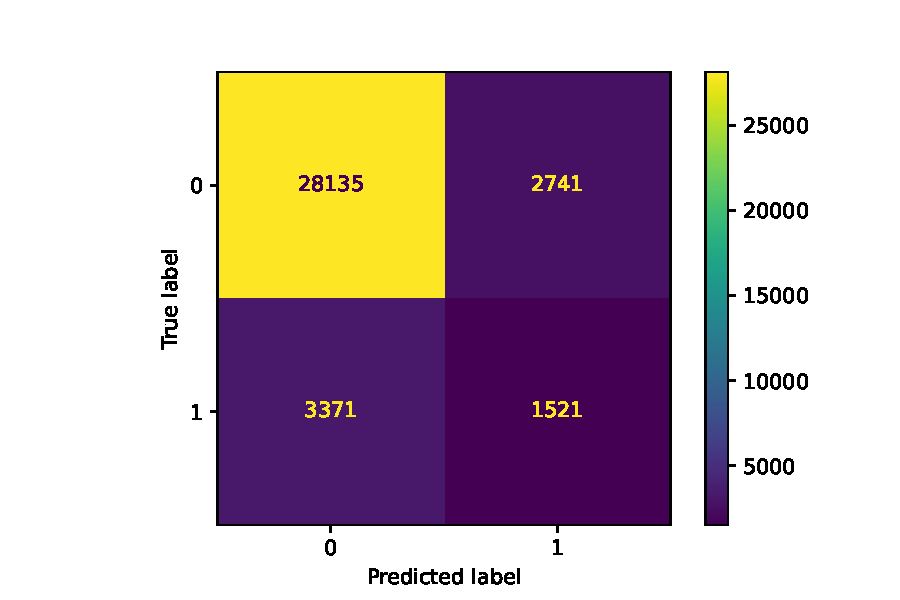
\includegraphics[width=0.5\textwidth]{img/tm_mlp_lbgfs_confusion_matrix.pdf}
	\caption{Confusion Matrix}
	\label{fig:confusion_matrix}
\end{figure}

As the final step of our data cleanup a column “voteSuccess” was added to the dataframe, calculating helpfulness of a review by dividing number of votes from the “votes”-column by quarters elapsed since the review was submitted. This was done to create a fairer indicator of helpfulness, since newer reviews would have had less time to accumulate helpfulness-votes and therefore appear less helpful.
%------------------------------------------------

\section{Findings}

Looking at our table of model test runs\ref{model_test_runs}, no model was fully able to predict, with any certainty, which reviews were helpful. The Count document-term matrix using an MLP classifier with the LBFGS algorithm on a neural network of 1 layer of 50 nodes, with a training-set size of 876132, reached the best performance, with a Youden’s Index of 0.25646. Comparatively, other classifiers did worse, with LinearSVC doing only slightly worse than LBFGS on smaller training-sets, and the Adam Solver MLP classifier doing slightly worse on bigger training-sets.

When comparing the performance metrics of the models using different types of input data, Count or TF-IDF, Count did remarkably better. This could be interpreted as Count doing better when facing a classification problem, since some terms that would normally help distinguish between the two groups likely being suppressed by the IDF, removing valuable terms. Further examination is required to discover if this is the case, and if so, if another approach to parameterizing our dataset, like Bi-Normal Separation\footnote\footnotetext{Jean-Thomas Baillargeon, Luc Lamontagne, and Étienne Marceau, 2018.} would perform better than Count.

Overall, our model was able to predict a helpful review in 1/3 of the cases, indicating that a more in-depth approach, possibly involving more features than the two currently provided, to training our model is required.

%------------------------------------------------
\section{Conclusion}
In this paper we have analyzed to what extent we can use classification models to predict the helpfulness of an Amazon review based on the review text and upvotes.

Based on the analysis we find that the features used are not sufficient in determining the helpfulness of a review when using common classification tools. The inclusion of several other features contained in our dataset would likely improve upon the predictive power of our models.

Solely classifying reviews based on term-frequency may not be enough to properly distinguish between helpful and unhelpful, as the review text can be nearly identical in both cases. This can be due to the fact that many reviews containing terms that would be labeled as helpful get lost in the large volume of unvoted reviews as seen in \figurename{\ref{fig:votes_distribution}}.


%----------------------------------------------------------------------------------------
%	REFERENCE LIST
%----------------------------------------------------------------------------------------

\begin{thebibliography}{99} % Bibliography - this is intentionally simple in this template
	\bibitem[scikit-learn LinearSVC]{sklearn:LinearSVC}
	\url{https://scikit-learn.org/stable/modules/generated/sklearn.svm.LinearSVC.html}
	\bibitem[scikit-learn MLPClassifier]{sklearn:MLPClassifier}
	\url{https://scikit-learn.org/stable/modules/generated/sklearn.neural_network.MLPClassifier.html}
	\bibitem[scikit-learn Count Vectorizer]
	\url{https://scikit-learn.org/stable/modules/generated/sklearn.feature_extraction.text.CountVectorizer.html}
	\bibitem[scikit-learn TF-IDF Vectorizer]
	\url{https://scikit-learn.org/stable/modules/generated/sklearn.feature_extraction.text.TfidfVectorizer.html}
	\bibitem[NLP Data Preprocessing]{NLP}
	\url{https://towardsdatascience.com/text-normalization-for-natural-language-processing-nlp-70a314bfa646}
	\url{https://scikit-learn.org/stable/modules/generated/sklearn.neural_network.MLPClassifier.html} \newblock {\em Human Nature}, 20:317--330.
	\bibitem[scikit-learn LogisticRegression]{sklearn:LogisticRegression}
	\url{https://scikit-learn.org/stable/modules/generated/sklearn.linear_model.LogisticRegression.html}
	\bibitem[Yves Rychener, 2018]{Yves:2018dg}
	Yves Rychener, Nicolas Zimmermann, Loïs Bilat
	\newblock Detecting Bias in Amazon reviews
	\url{https://ada-lyn.github.io/}
	\bibitem[Jean-Thomas Baillargeon, Luc Lamontagne, and Étienne Marceau.]
	\newblock Weighting Words Using Bi-Normal Separation for Text Classification Tasks with Multiple Classes. ResearchGate, 2019
	\bibitem [Dirk Hovy, Shannon L. Spruit]{censorship}
	\newblock The Social Impact of Natural Language Processing. Dirkhovy.com, 2018.
\end{thebibliography}

%----------------------------------------------------------------------------------------

\end{document}
